\documentclass[11pt]{article}

\author{Math 1060}
\date{Due Friday, October 3 by 11:59pm} 
\title{Homework 3}

\usepackage{graphicx,xypic}
\usepackage{amsthm}
\usepackage{amsmath,amssymb}
\usepackage{amsfonts}
\usepackage{xcolor}
\usepackage[margin=1in]{geometry}
\usepackage[shortlabels]{enumitem}
\newtheorem{problem}{Problem}
\renewcommand*{\proofname}{{\color{blue}Solution}}


\setlength{\parindent}{0pt}
\setlength{\parskip}{1.25ex}


\begin{document}

\maketitle


% DON'T LEAVE THIS BLANK! 
{\bf\Large Your Name:} 

% DON'T FORGET YOUR COLLABORATORS! 
Collaborator names: 


\vspace{.3in}
Topics covered: curvature, Frenet frame, fundamental theorem of space curves, Gauss map

Instructions {\bf (read these carefully!)}: 
\begin{itemize}
\item This assignment must be submitted on Gradescope by the due date. 
\item If you collaborate with other students (which is encouraged!), please list your collaborators above. 
\item Homework is graded anonymously, so please avoid putting your name on every page of the assignment.
\item If you are stuck, please ask for help (from me, Nathan, or a classmate). Use Campuswire!  
\item You may freely use any fact proved in class (mention it in the appropriate spot). You can also use basic facts from calculus or linear algebra without justification (but be sure to say what fact you're using and where). You may not freely use facts from the book, and generally your source material for completing the assignent should be the lecture, rather than the book (particularly when there is some discrepancy between these). 
\item Please restrict your solution to each problem to a single page. Usually solutions can be even shorter than that. If your solution is very long, you should think more about how to express it concisely.
\end{itemize}
\pagebreak 


\begin{problem}
Write down a linear system of differential equations in functions $f_1,\ldots,f_6$ that is satisfied by $f_1=T\cdot N$, $f_2=T\cdot B$, $f_3=N\cdot B$, $f_4=T\cdot T$, $f_5=N\cdot N$, $f_6=B\cdot B$ when $T,N,B$ satisfy the Frenet equations.\footnote{Hint: differentiate these dot product functions, and express the answer back in terms of these functions. The final answer should be a system of differential equations involving $f_1,\ldots,f_6$, and \emph{not(!)}  involving $T,N,B$.} Verify that the functions $f_1=f_2=f_3=0$ and $f_4=f_5=f_6=1$ is a solution to your system of differential equations.
\end{problem}

\begin{proof}

\end{proof}

\pagebreak


\begin{problem}
Use the previous problem to give a careful proof of the fundamental theorem of space curves, finishing the argument from class. (Specifically, show for every $\kappa:[0,L]\to[0,\infty)$ and $\tau:[0,L]\to\mathbb R$, there is a unit speed curve with curvature $\kappa$ and torsion $\tau$.) 
\end{problem}

\begin{proof}

\end{proof}

\pagebreak

\begin{problem}
Let $c:[0,L]\to\mathbb R^2$ be a unit-speed plane curve, and assume $c(0)=c(L)$ and $c'(0)=c'(L)$. Write $c'(t)=(\cos\theta(t),\sin\theta(t))$, where $\theta:[0,L]\to\mathbb R$. Then $\frac{1}{2\pi}\big(\theta(L)-\theta(0)\big)$ is an integer, called the turning number of $\alpha$. Compute the turning number of the following curves.\footnote{Hint: Fix a direction, e.g.\ $(1,0)$ and find all the points on the curve where the tangent vector points in the direction of $(1,0)$ (not its negative). Then count these points with sign...}
\begin{center}
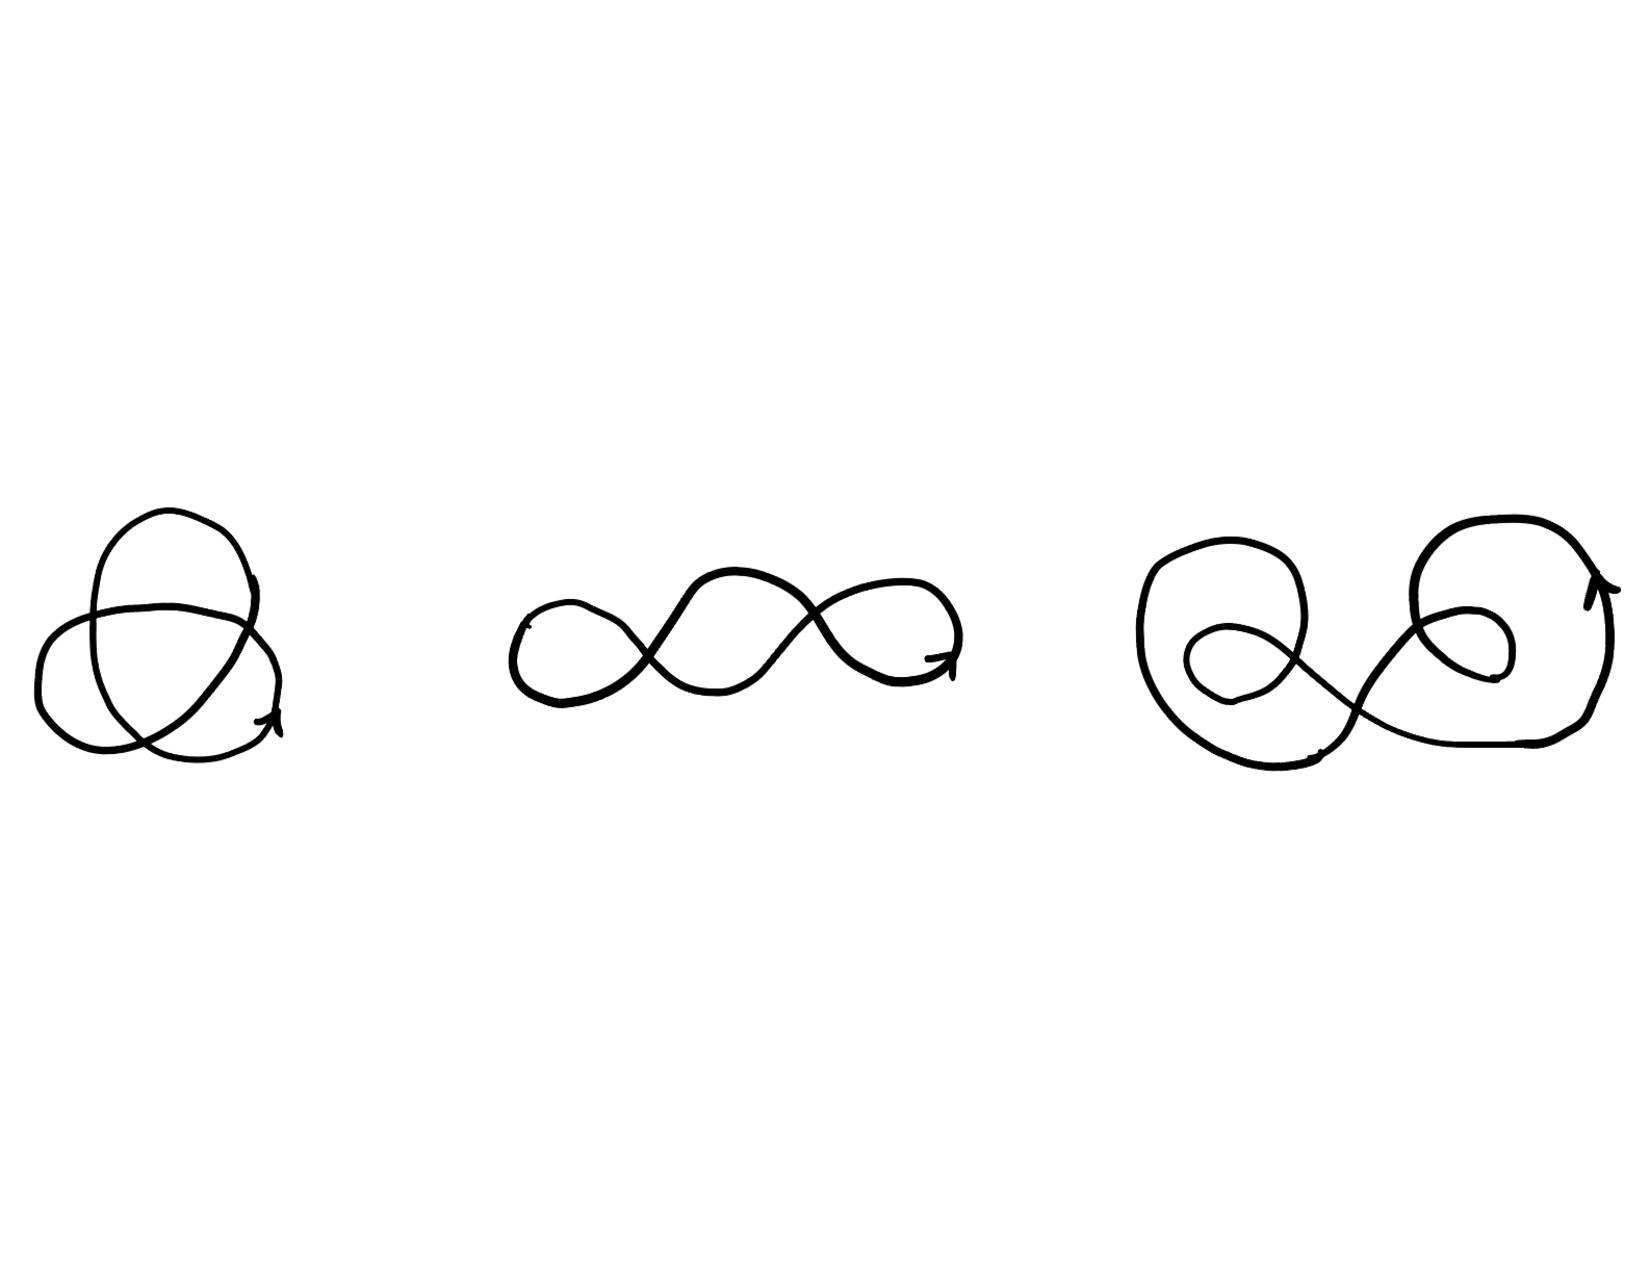
\includegraphics[scale=.5]{tn.pdf}
\end{center}
\end{problem}

\begin{proof}

\end{proof}

\pagebreak

\begin{problem}
For the hyperboloid $\phi(u,v)=(u,v,v^2-u^2)$ with unit normal $N=\phi_u\times\phi_v/|\phi_u\times \phi_v|$, compute $DN_p$ at $p=(0,0,0)$. 
\end{problem}

\begin{proof}

\end{proof}

\pagebreak

\begin{problem}
Describe the image of the Gauss map of the following surfaces. Do \emph{not} compute using a chart. Instead, reason geometrically.
\begin{enumerate}[(a)]
\item Paraboloid $z=x^2+y^2$. 
\item Hyperboloid $x^2+y^2-z^2=1$. 
\end{enumerate} 
\end{problem}

\begin{proof}

\end{proof}

\pagebreak


\begin{problem}
In this problem you prove the spectral theorem for self-adjoint linear operators $A:\mathbb R^2\to\mathbb R^2$ (using differential geometry!). \footnote{Remark: This special case of the theorem is the most important case for us in the course.}

Consider the composition $f\circ c$, where $c:[0,2\pi]\to\mathbb R^2$ is the standard parameterization of the unit circle, and $f:\mathbb R^2\to\mathbb R$ is defined by $f(p)=\langle A(p), p\rangle$. 
\begin{enumerate}[(a)]
\item Compute $(f\circ c)'(t)$ and prove that $t$ is a critical point of $f\circ c$ if and only if $c(t)$ is an eigenvector of $A$. Relate the corresponding eigenvalue to $f$. 
\item Use facts from calculus to deduce that either $A$ is a scalar matrix or $A$ has two distinct eigenvalues. 
\item Prove that there exist a pair of eigenvectors for $A$ that form an orthonormal basis for $\mathbb R^2$. \footnote{Hint: this is just a linear algebra exercise. Make sure to use the hypothesis...}
\end{enumerate} 
\end{problem}

\begin{proof}

\end{proof}






\end{document}